\chapter{Otras Gráficas}
\label{chap:sinqos}

\begin{figure}[!ht]
    \centering
    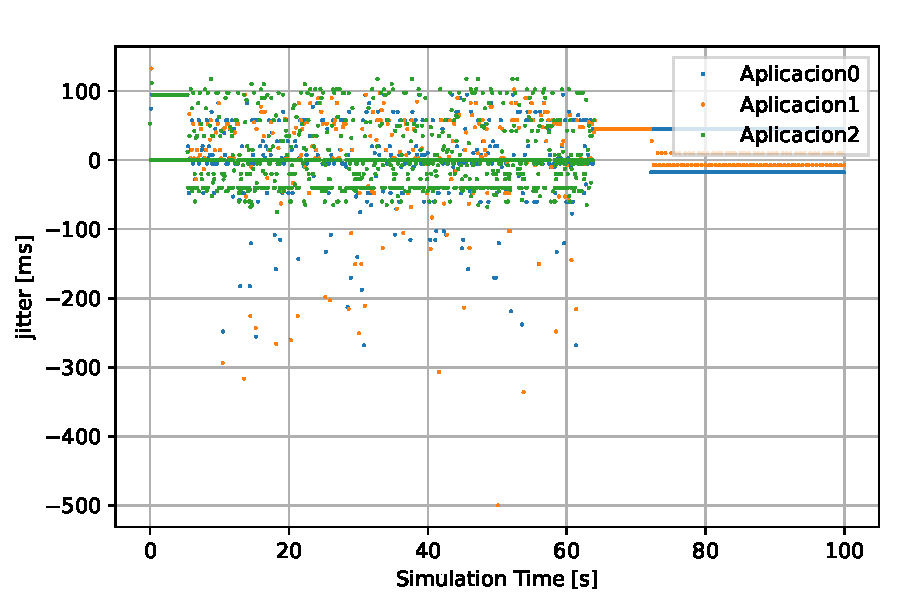
\includegraphics{graficas/sinQoS/jitter_SinQoS.pdf}
    \caption{Jitter a partir retardo extremo a extremo del router sin QoS}
    \label{fig:sinqos_jitter}
\end{figure}

\begin{figure}
    \centering
    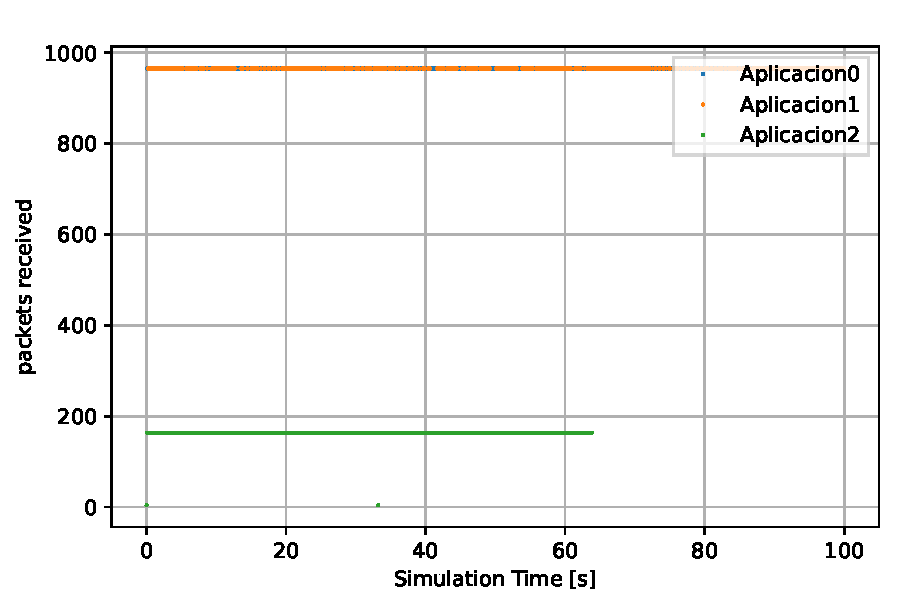
\includegraphics{graficas/sinQoS/packetsReceived_sinQoS.pdf}
    \caption{Paquetes recibidos en el servidor sin QoS}
    \label{fig:sinqos_pktreceived}
\end{figure}

\begin{figure}
    \centering
    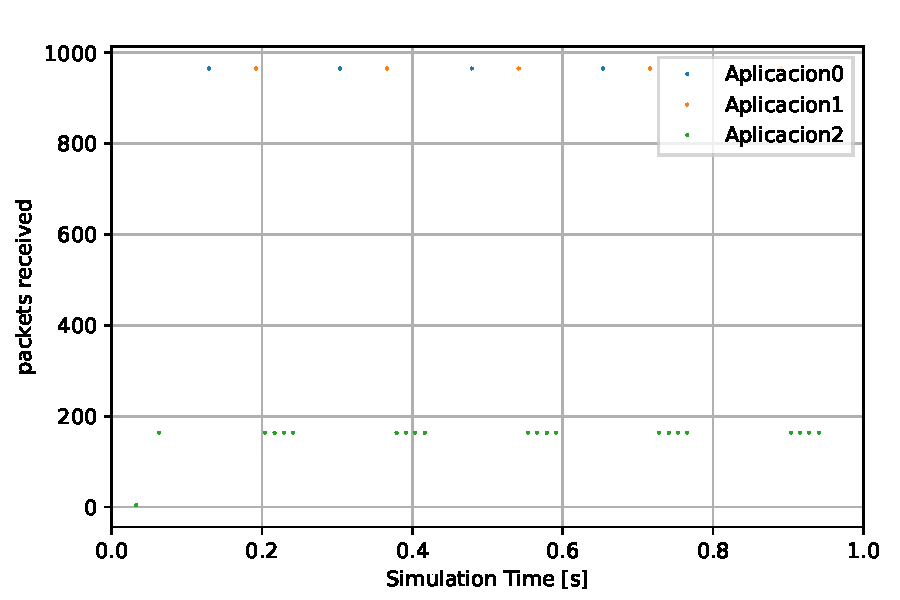
\includegraphics{graficas/sinQoS/packetsReceived_sinQoS_1.pdf}
    \caption{Paquetes recibidos en el servidor sin QoS intervalo 0-1}
    \label{fig:sinqos_pktreceived01}
\end{figure}

\begin{figure}
    \centering
    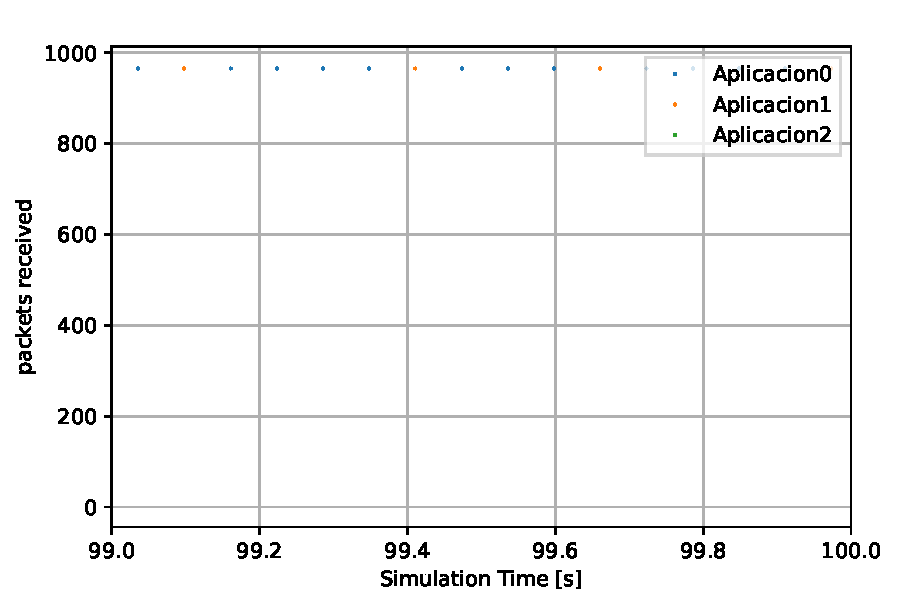
\includegraphics{graficas/sinQoS/packetsReceived_sinQoS_99.pdf}
    \caption{Paquetes recibidos en el servidor sin QoS intervalo 99-100}
    \label{fig:sinqos_pktreceived99100}
\end{figure}


\begin{figure}[!ht]
    \centering
    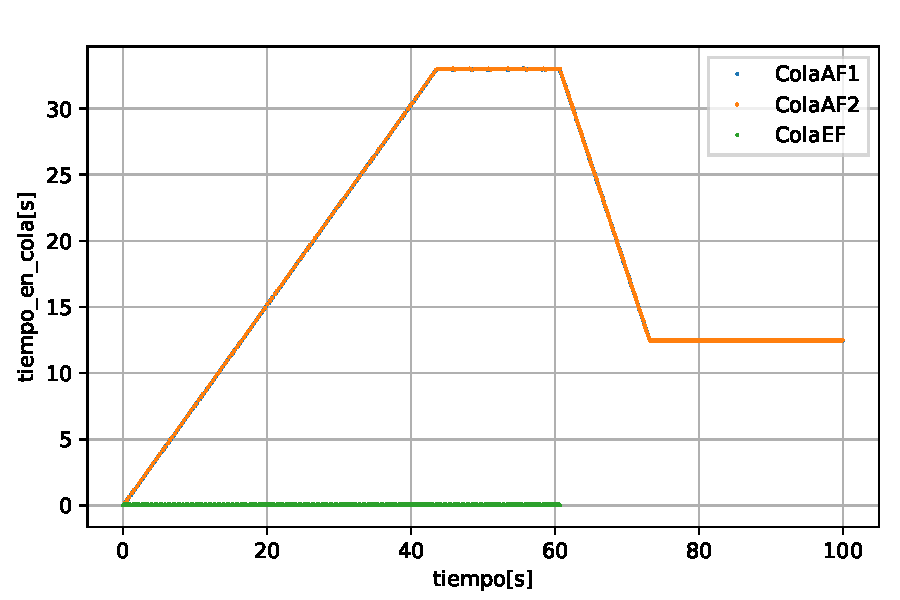
\includegraphics{graficas/DropTail/tiempo_en_cola_droptail.pdf}
    \caption{Tiempo encolado droptail}
    \label{fig:droptail_time}
\end{figure}

\begin{figure}
    \centering
    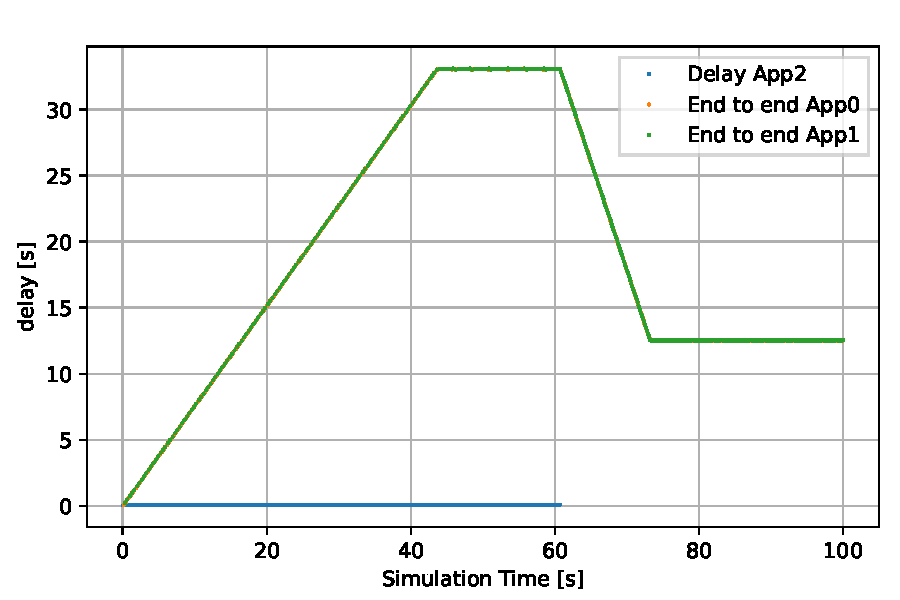
\includegraphics{graficas/DropTail/delay_DT.pdf}
    \caption{Delay extremo a extremo con droptail}
    \label{fig:sinqos_pktreceived99100}
\end{figure}

\begin{figure}
    \centering
    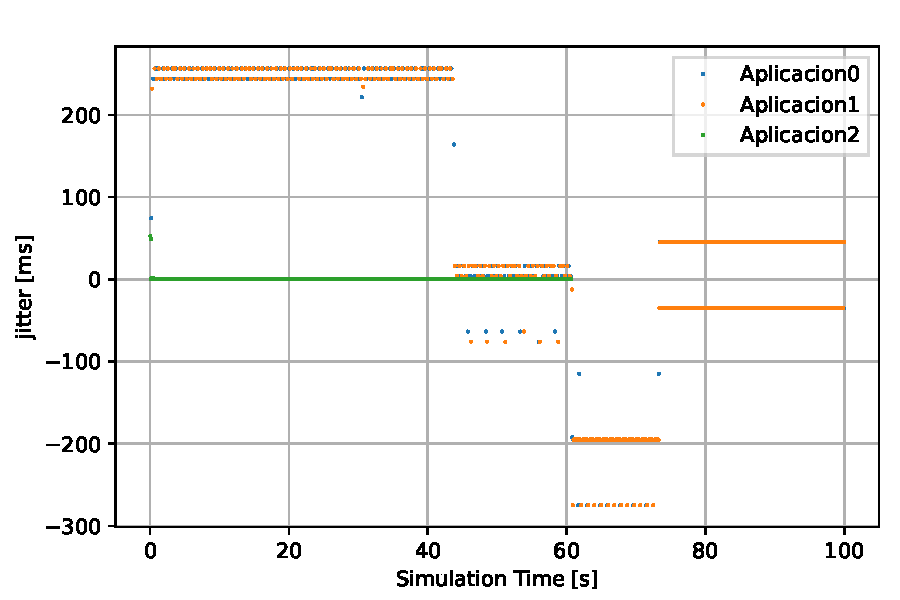
\includegraphics{graficas/DropTail/jitter_DT.pdf}
    \caption{Jitter a partir retardo extremo a extremo droptail}
    \label{fig:sinqos_pktreceived99100}
\end{figure}

\begin{figure}
    \centering
    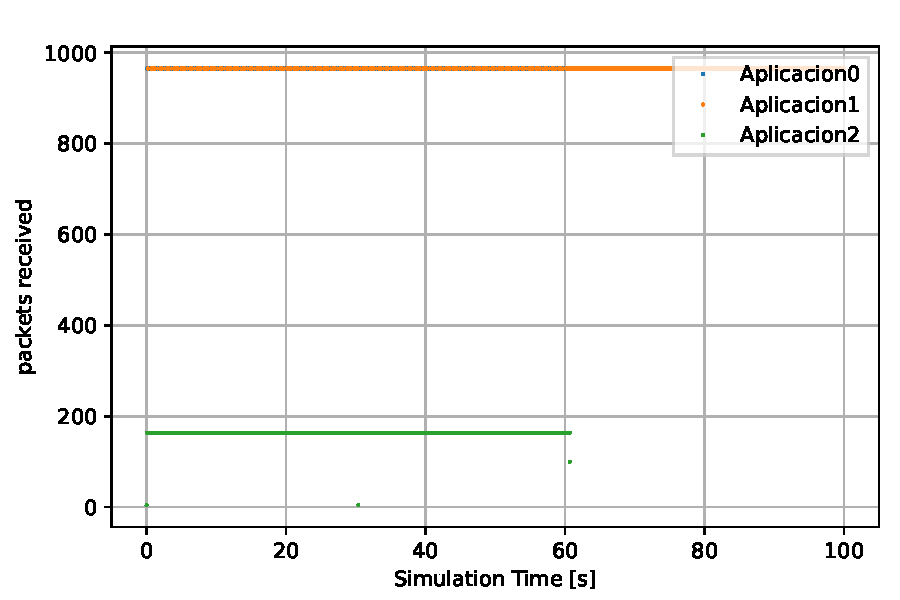
\includegraphics{graficas/DropTail/packetsReceived_DT.pdf}
    \caption{Paquetes recibidos en el servidor droptail}
    \label{fig:sinqos_pktreceived99100}
\end{figure}

\begin{figure}
    \centering
    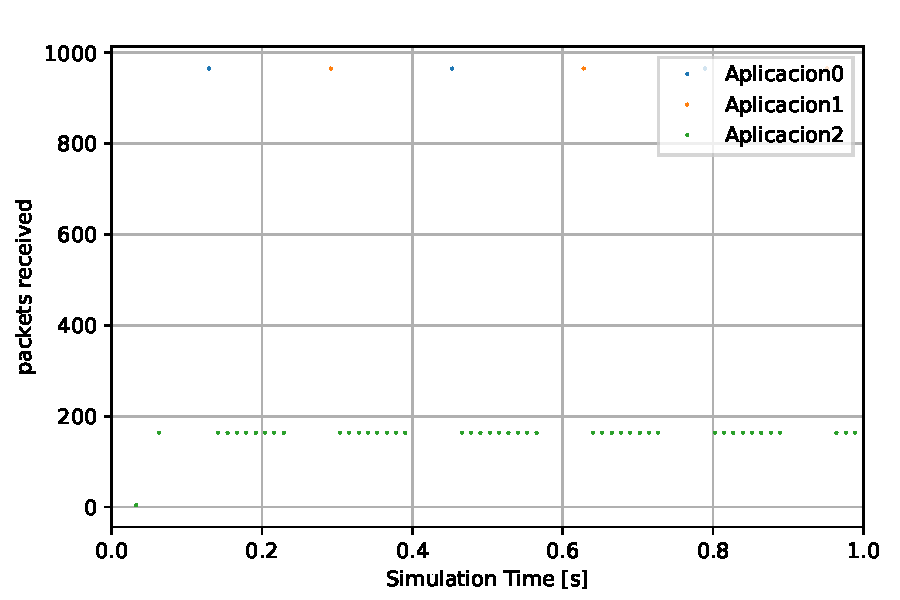
\includegraphics{graficas/DropTail/packetsReceived_DT_1.pdf}
    \caption{Paquetes recibidos en el sevidor droptail intervalo 0-1 }
    \label{fig:sinqos_pktreceived99100}
\end{figure}

\begin{figure}
    \centering
    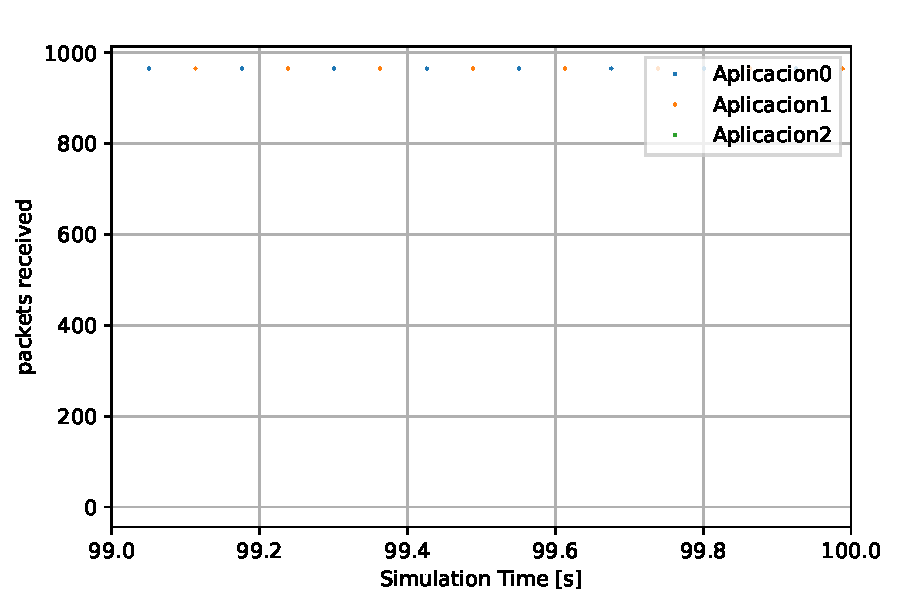
\includegraphics{graficas/DropTail/packetsReceived_DT_99.pdf}
    \caption{Paquetes recibidos en el servidor droptail intervalo 99-100}
    \label{fig:sinqos_pktreceived99100}
\end{figure}


\begin{figure}[!ht]
    \centering
    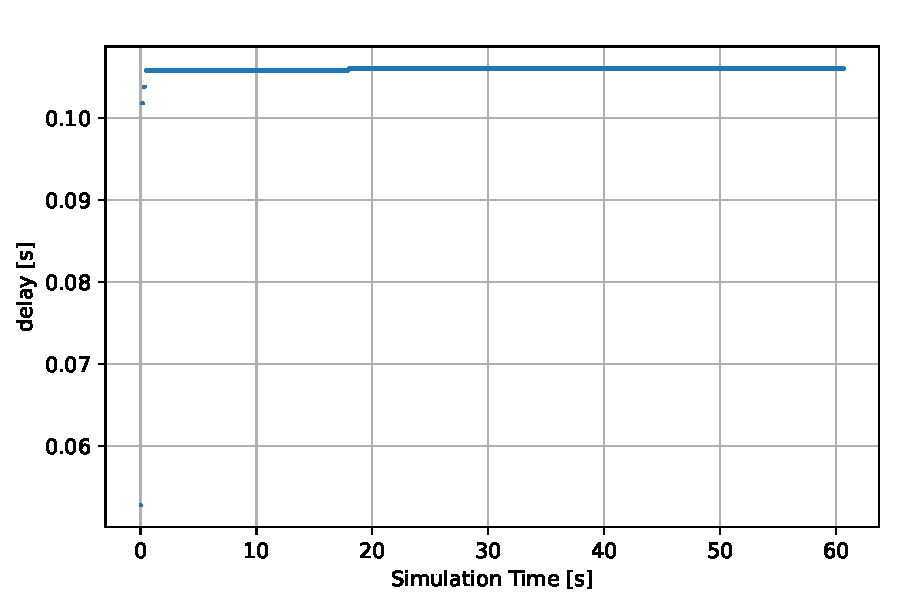
\includegraphics{graficas/WRR/delay_wrr.pdf}
    \caption{Retardo extremo a extremo WRR16}
    \label{fig:sinqos_pktreceived99100}
\end{figure}

\begin{figure}
    \centering
    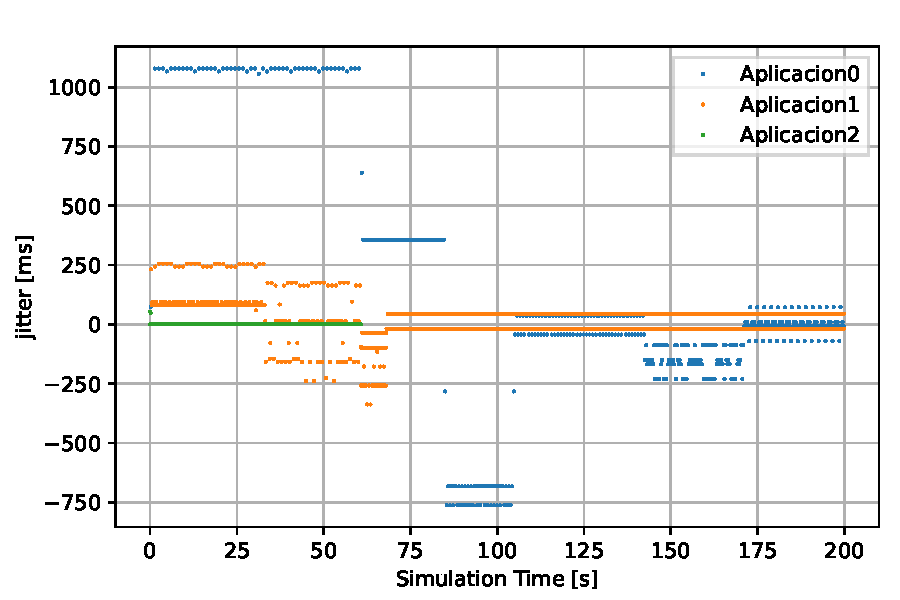
\includegraphics{graficas/WRR/jitter_WRR.pdf}
    \caption{Jitter a partir retardo extremo a extremo WRR16}
    \label{fig:sinqos_pktreceived99100}
\end{figure}

\begin{figure}
    \centering
    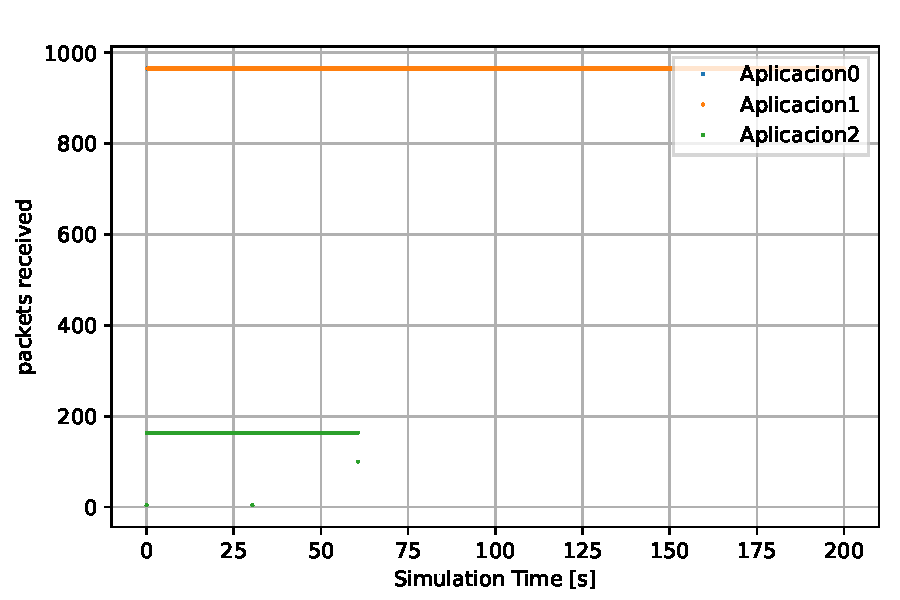
\includegraphics{graficas/WRR/packetsReceived_WRR.pdf}
    \caption{Paquetes recibidos en el servidor con WRR16}
    \label{fig:sinqos_pktreceived99100}
\end{figure}

\begin{figure}
    \centering
    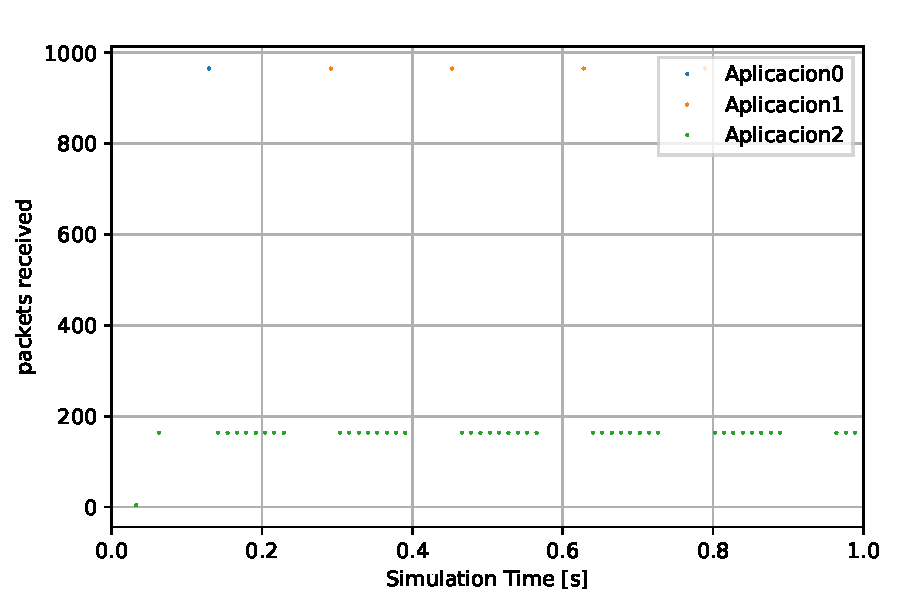
\includegraphics{graficas/WRR/packetsReceived_WRR_1.pdf}
    \caption{Paquetes recibidos en el servidor con WRR16 intervalo 0-1}
    \label{fig:sinqos_pktreceived99100}
\end{figure}

\begin{figure}
    \centering
    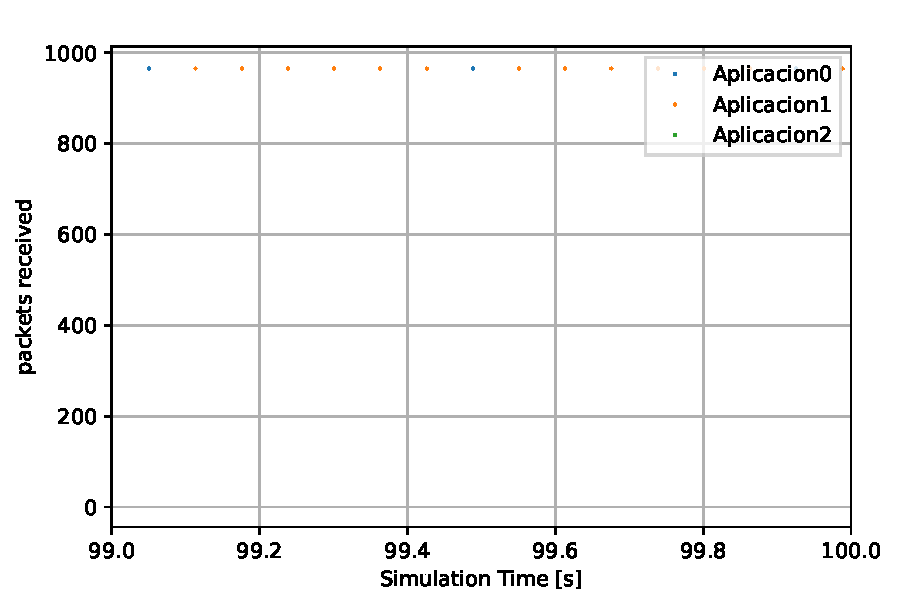
\includegraphics{graficas/WRR/packetsReceived_WRR_99.pdf}
    \caption{Paquetes recibidos en el servidor con WRR16 intervalo 99-100}
    \label{fig:sinqos_pktreceived99100}
\end{figure}

\begin{figure}
    \centering
    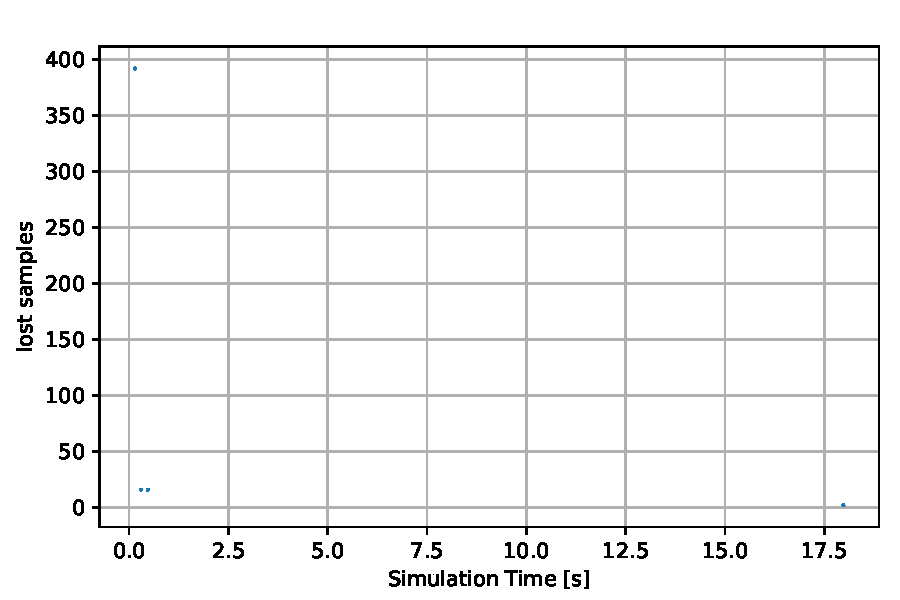
\includegraphics{graficas/WRR/muestras_perdidas_wrr.pdf}
    \caption{Muestras perdidas WRR16}
    \label{fig:sinqos_pktreceived99100}
\end{figure}


\begin{figure}[!ht]
    \centering
    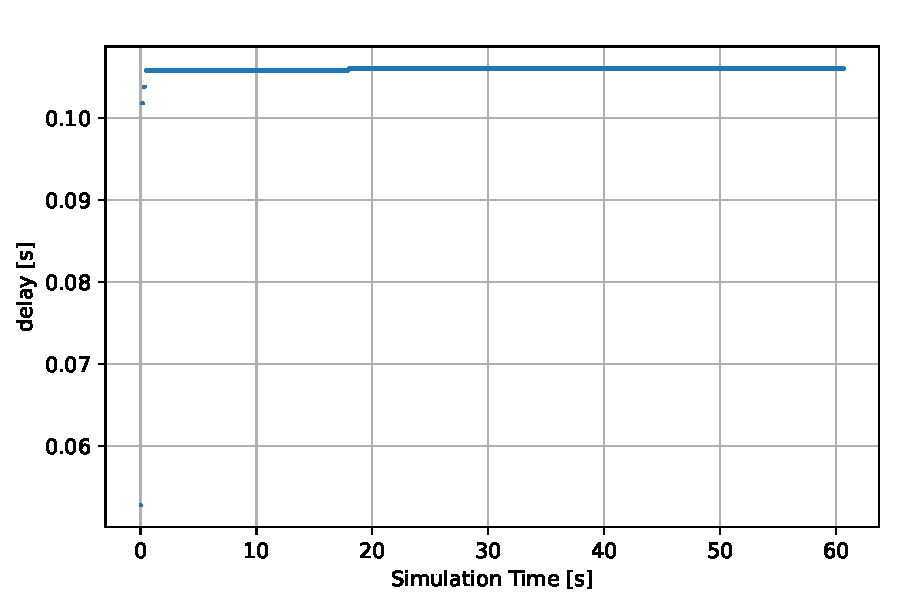
\includegraphics{graficas/RED/delay_red.pdf}
    \caption{Retardo extremo a extremo RED}
    \label{fig:sinqos_pktreceived99100}
\end{figure}

\begin{figure}
    \centering
    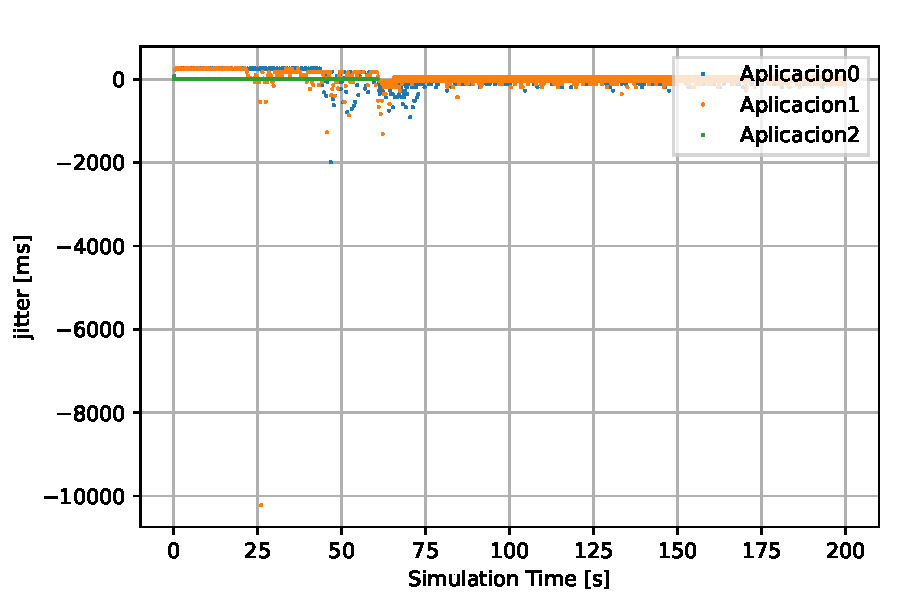
\includegraphics{graficas/RED/jitter_RED.pdf}
    \caption{Jitter a partir retardo extremo a extremo RED}
    \label{fig:sinqos_pktreceived99100}
\end{figure}

\begin{figure}
    \centering
    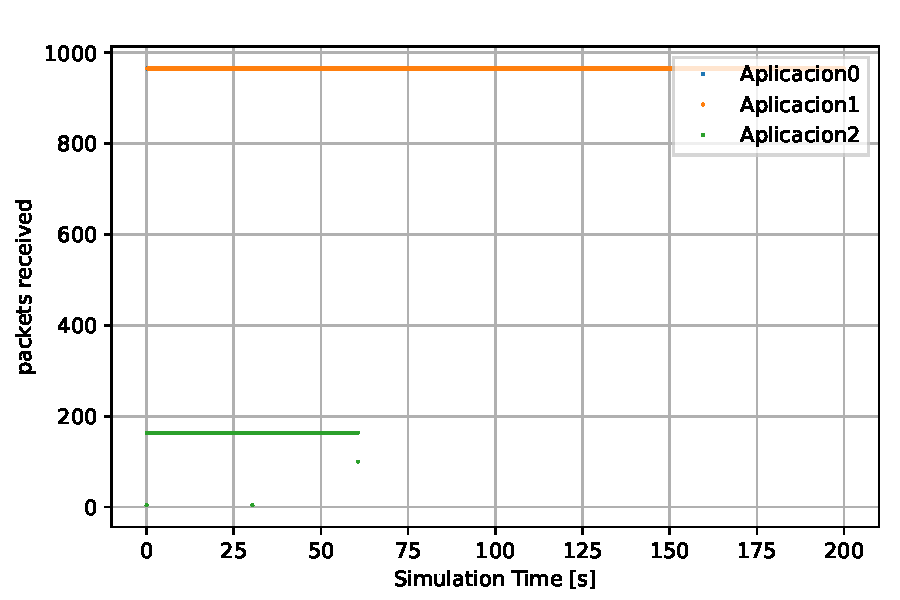
\includegraphics{graficas/RED/packetsReceived_RED.pdf}
    \caption{Paquetes recibidos en el servidor con RED}
    \label{fig:sinqos_pktreceived99100}
\end{figure}

\begin{figure}
    \centering
    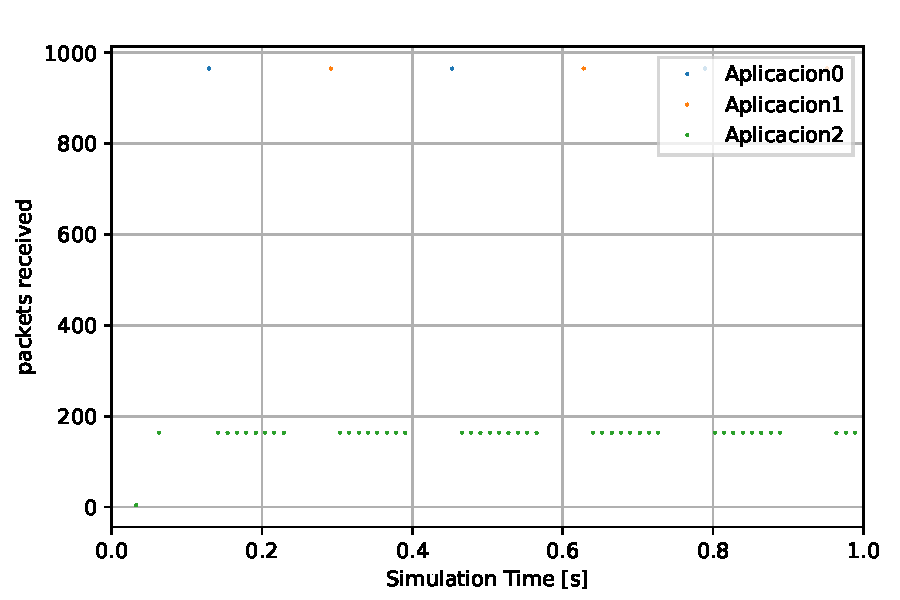
\includegraphics{graficas/RED/packetsReceived_RED_1.pdf}
    \caption{Paquetes recibidos en el servidor con RED intervalo 0-1}
    \label{fig:sinqos_pktreceived99100}
\end{figure}

\begin{figure}
    \centering
    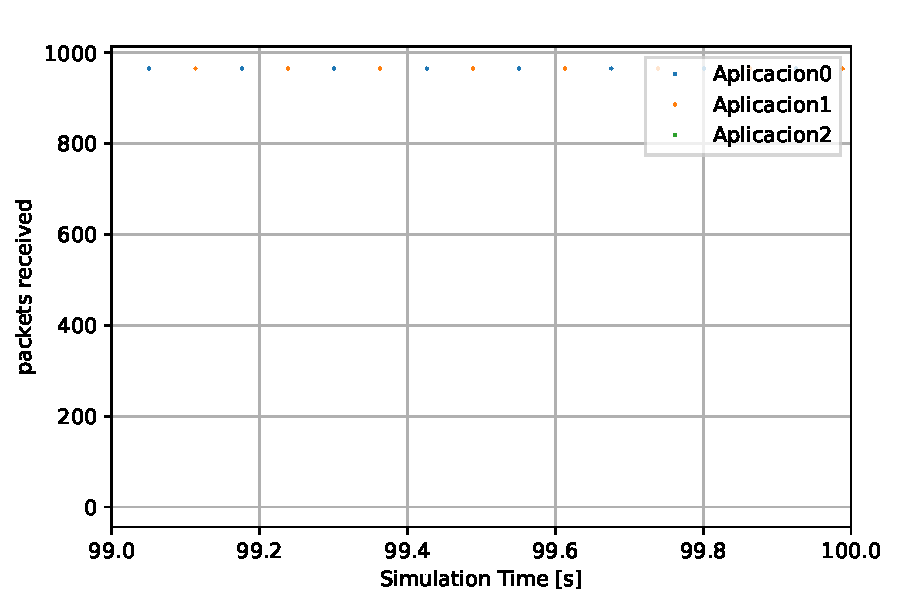
\includegraphics{graficas/RED/packetsReceived_RED_99.pdf}
    \caption{Paquetes recibidos en el servidor con RED intervalo 99-100}
    \label{fig:sinqos_pktreceived99100}
\end{figure}

\begin{figure}
    \centering
    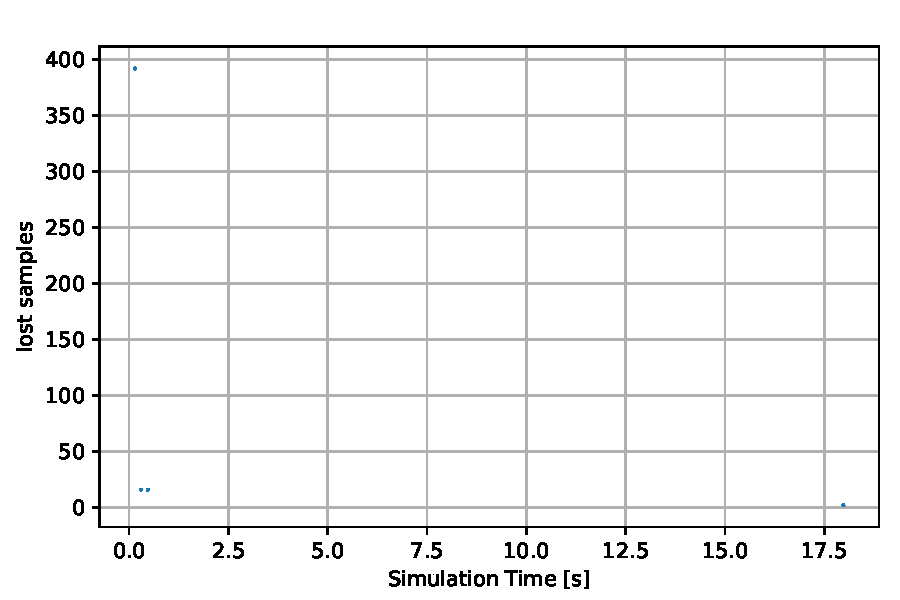
\includegraphics{graficas/RED/muestras_perdidas_red.pdf}
    \caption{Muestras perdidas con RED}
    \label{fig:sinqos_pktreceived99100}
\end{figure}


